\documentclass[11pt,a4paper]{article}
\usepackage[margin=1in]{geometry}
\usepackage{graphicx}
\usepackage{booktabs}
\usepackage{amsmath}
\usepackage{hyperref}
\usepackage[numbers]{natbib}
\usepackage{listings}
\usepackage{xcolor}
\usepackage{float}
\usepackage{subcaption}

% Code listing style
\lstset{
    basicstyle=\ttfamily\small,
    keywordstyle=\color{blue},
    commentstyle=\color{gray},
    stringstyle=\color{orange},
    frame=single,
    breaklines=true,
    language=Python,
    showstringspaces=false
}

\title{Regime-Aware Experience Replay for Deep Reinforcement Learning in Portfolio Optimization}
\author{Prince Alexander John \\ University of Birmingham \\ School of Computer Science \\ \textit{Supervised by Dr Tao Chen}}
\date{March 2026}

\begin{document}
\maketitle

\begin{abstract}
Portfolio optimization under changing market conditions remains a significant challenge in quantitative finance. Traditional methods assume stationary return distributions, however markets exhibit distinct regimes such as bull, bear and sideways phases that invalidate these assumptions. We investigate whether regime-aware experience replay can improve deep reinforcement learning for portfolio management. Drawing from \citet{nixon2025regime}, who demonstrated benefits from regime-conditioned observations for on-policy algorithms, we modify the replay buffer sampling strategy for off-policy methods. We evaluate four algorithms (PPO, SAC, TD3, Rainbow DQN) across five replay strategies using 228 runs across seven experiments. TD3 with standard replay achieves the highest Sharpe ratio of $+0.632$, significantly outperforming the S\&P 500 ($-0.006$) during the challenging 2022--2023 test period. We discover that SAC is fundamentally incompatible with regime-aware replay due to entropy bias from non-uniform sampling. This is a novel finding with implications for algorithm selection in regime-switching environments. These results demonstrate that algorithm choice dominates strategy choice, while regime-aware replay benefits deterministic policy algorithms but harms entropy-regularised methods.
\end{abstract}

\vspace{0.5em}
\noindent\textit{A companion Technical Appendix containing full results, statistical tests, hyperparameters, code listings and bug documentation is available at: \url{https://git.cs.bham.ac.uk/projects-2025-26/pxx276/-/blob/main/report/appendix.pdf}}

\section{Introduction}

Portfolio optimization, allocating capital across financial assets to maximize risk-adjusted returns, has long challenged practitioners and researchers. Traditional approaches such as Markowitz mean-variance optimization \citep{markowitz1952} assume stationary return distributions, yet financial markets transition between distinct regimes with different volatility levels, correlations and return dynamics \citep{hamilton1989regime, ang2002regime}.

Deep reinforcement learning has emerged as a promising approach to portfolio management \citep{yang2020deep, drl_survey2024}, but standard DRL methods implicitly assume training experiences are drawn from a single distribution. Market regimes exhibit qualitatively different dynamics \citep{hamilton1989regime} and an agent trained predominantly on bull market data may fail when conditions shift.

Nixon Raj \citep{nixon2025regime} demonstrated that adding regime probabilities derived from a Hidden Markov Model to the observation space improves PPO performance by modifying what the agent \textit{observes}. We propose a complementary technique: modifying how the agent \textit{samples past experiences} during training via regime-aware replay strategies.

To our knowledge, this is the first systematic investigation of regime-aware replay buffer sampling for off-policy DRL in portfolio optimization. Our contributions:

\begin{enumerate}
    \item We discover that replay strategy effects are dependent on the algorithm. Regime-aware replay is tolerated by TD3 but fundamentally incompatible with SAC due to entropy bias, revealing that replay modifications must respect learning algorithm assumptions.

    \item We design five regime-aware replay strategies and conduct 228 runs across seven experiments with Bonferroni-corrected statistical testing, providing the first systematic evaluation of replay-algorithm interactions in financial DRL.

    \item We demonstrate that TD3 with standard replay achieves the best test performance (Sharpe +0.632), substantially outperforming all passive baselines during the challenging 2022–2023 period.

    \item We show the approach is robust to imperfect regime detection (E3), detection method is immaterial (E5) and that 400k timesteps is the optimal training duration, balancing fit and generalisation (E7).
\end{enumerate}


\section{Background and Related Work}
\label{sec:background}

\subsection{Deep Reinforcement Learning for Portfolio Management}

DRL frames portfolio management as sequentially making decisions under uncertainty \citep{mnih2015dqn, hoque2025review}. \textit{On-policy} methods such as PPO \citep{schulman2017ppo} discard experiences after each update, while \textit{off-policy} methods such as SAC \citep{haarnoja2018sac} and TD3 \citep{fujimoto2018td3} store experiences in a replay buffer for reuse. This is particularly attractive given scarce financial data. TD3 has been independently validated for portfolio optimisation \citep{jiang2024td3portfolio} and large-scale evaluations show that feature selection significantly affects downside risk \citep{ayari2025feature}. A recent survey \citep{drl_survey2024} documents competitive performance against traditional methods, though concerns about overfitting and regime-dependence persist.

\subsection{Experience Replay in Off-Policy Learning}

Experience replay \citep{mnih2015dqn} stores transitions $(s_t, a_t, r_t, s_{t+1})$ and samples mini-batches for training, breaking temporal correlations. Prioritized Experience Replay (PER) \citep{schaul2016per} samples proportionally to TD error magnitude but does not account for the \textit{source} of experiences - a critical limitation in non-stationary environments. A recent survey documents the exponential growth in replay research \citep{neves2025er_survey}. Standard uniform sampling introduces subtle bias by favouring older transitions \citep{yenicesu2024cuer}, and non-uniform sampling can degrade actor-critic methods. \citet{saglam2023actor} proved that high-TD-error transitions produce biased policy gradients, and \citet{wang2019ere} found SAC particularly sensitive to replay distribution changes. Our work extends this by introducing \textit{regime-aware} sampling that considers the market regime from which each experience originated.

\subsection{Market Regime Detection}

Hamilton's Markov-switching models \citep{hamilton1989regime} established regime detection as hidden Markov processes with discrete latent states. \citet{ang2002regime} demonstrated that regime-awareness improves portfolio allocation, and ensemble methods combining HMMs with technical indicators achieve robust classification \citep{gupta2025forest}. We employ a rule-based detector using moving average crossovers and volatility thresholds as default, comparing against an HMM classifier in experiment E5.

\subsection{Related Work: Nixon Raj (2025)}

Nixon Raj \citep{nixon2025regime} augments the agent's observation space with HMM-derived regime probabilities, demonstrating improved PPO and Transformer-based performance. Our approach is complementary. Rather than modifying observations, we modify replay sampling for off-policy algorithms while requiring no architectural changes. The two could be combined. A key concern is algorithm interaction: SAC's entropy term assumes samples reflect the true state-action distribution, and non-uniform sampling may bias entropy estimates. This is a hypothesis we investigate in Section~\ref{sec:results}.



\section{Methodology}
\label{sec:methodology}

\subsection{Problem Formulation}

We formulate portfolio optimization as an MDP $(S, A, R, P, \gamma)$ over $n=5$ assets. The state $s_t \in \mathbb{R}^d$ concatenates technical indicators, current portfolio weights $w_t \in \mathbb{R}^n$ and normalized portfolio value $\tilde{V}_t = V_t / V_0 - 1$. Actions $a_t \in [-1, 1]^n$ are transformed into valid weights via softmax:
\begin{equation}
    w_{t+1}^{(i)} = \frac{\exp(a_t^{(i)})}{\sum_{j=1}^{n} \exp(a_t^{(j)})}
\end{equation}
ensuring non-negative weights that sum to one (no short-selling). The reward function balances returns, transaction costs and risk:
\begin{equation}
    r_t = R_p - \lambda_{\text{cost}} \cdot \frac{c_t}{V_{t-1}} - \lambda_{\text{risk}} \cdot \max(0,\; \text{DD}_t - \text{DD}_{\text{thresh}})
\end{equation}
where $R_p = (V_t - V_{t-1})/V_{t-1}$ is portfolio return, $c_t$ is transaction cost (10 bps on traded value), $\text{DD}_t$ is drawdown from peak, $\lambda_{\text{cost}} = 1.0$, $\lambda_{\text{risk}} = 0.1$, and $\text{DD}_{\text{thresh}} = 0.10$. The risk penalty weight is deliberately smaller than the cost penalty to avoid overly conservative policies. Episodes span 252 trading days with \$1M initial capital.

\subsection{Algorithms}

We evaluate four algorithms spanning on-policy and off-policy paradigms, since regime-aware replay only applies to off-policy methods with a replay buffer. \textbf{PPO} \citep{schulman2017ppo} is on-policy and serves as a control, receiving regime information via observation augmentation with one-hot regime indicators \citep{nixon2025regime} rather than replay modification. \textbf{SAC} \citep{haarnoja2018sac} maximizes $J(\pi) = \mathbb{E}[\sum_t r_t + \alpha \mathcal{H}(\pi(\cdot|s_t))]$; the entropy term $\mathcal{H}$ assumes replay samples reflect the true state-action distribution. \textbf{TD3} \citep{fujimoto2018td3} uses twin Q-networks, delayed policy updates and target smoothing; as a deterministic policy method without an entropy term, it is less sensitive to replay distribution changes. \textbf{Rainbow DQN} \citep{hessel2018rainbow} combines distributional RL, dueling networks and double Q-learning over a discrete action space.


\subsection{Regime-Aware Experience Replay}

Standard experience replay \citep{mnih2015dqn} samples uniformly, but financial training data is regime-imbalanced: bull markets dominate while bear episodes are underrepresented. Our approach partitions the replay buffer by market regime. Each transition is tagged with $z_t \in \mathcal{Z} = \{\text{bull}, \text{bear}, \text{sideways}\}$ and placed in the corresponding sub-buffer $\mathcal{B}_z$. At training time, we control the sampling distribution $P(z)$ using five strategies (Table~\ref{tab:strategies}).

\begin{table}[h]
\centering
\small
\caption{Regime-aware replay sampling strategies. $|\mathcal{B}_z|$ denotes transitions stored for regime $z$, $K=3$ regimes, and $\bar{\delta}_z$ is mean absolute TD error for regime $z$.}
\label{tab:strategies}
\begin{tabular}{@{}llp{5cm}@{}}
\toprule
\textbf{Strategy} & \textbf{Sampling Probability} & \textbf{Hypothesis} \\
\midrule
Standard & $P(z) \propto |\mathcal{B}_z|$ & Uniform baseline; equivalent to standard replay \\
Balanced & $P(z) = 1/K$ & Equal regime representation prevents bias toward dominant market conditions \\
Current-focused & $P(z_{\text{curr}}) = 0.6$, $P(z_{\text{other}}) = 0.2$ & Prioritizing the current regime improves immediate adaptation \\
Inverse-frequency & $P(z) \propto 1/|\mathcal{B}_z|$ & Oversampling rare regimes (esp.\ bear markets) improves robustness \\
Adaptive & $P(z) \propto \bar{\delta}_z$ & Focusing on regimes with high TD errors targets where the agent struggles most \\
\bottomrule
\end{tabular}
\end{table}

The \textit{adaptive} strategy tracks TD errors per regime using an exponential moving average (EMA, $\alpha = 0.99$):
\begin{equation}
    \bar{\delta}_z \leftarrow \alpha \cdot \bar{\delta}_z + (1 - \alpha) \cdot \frac{1}{|B|} \sum_{i \in B_z} |\delta_i|
\end{equation}
making sampling responsive to the agent's evolving learning state. Our approach is related to PER \citep{schaul2016per} but operates at regime-level granularity; the two are orthogonal, and our Rainbow implementation combines both.

We do not apply importance sampling (IS) corrections for non-uniform sampling. This is supported by multiple findings: uncorrected non-uniform methods match IS-corrected alternatives \citep{fedus2020replay}. Non-uniform sampling is equivalent to a modified loss function, making IS weights unnecessary \citep{fujimoto2020equivalence}. Stratified replay, the closest analogue to our approach, corrects multiplicity bias without IS \citep{daley2021stratified} and full IS corrections cause variance explosion \citep{munos2016retrace}. Our regime-level reweighting across three bins is substantially milder than transition-level PER.

\subsection{Experimental Design}

\textbf{Asset universe and data.} Five ETFs spanning equities (SPY, QQQ), bonds (TLT), gold (GLD) and cash (BIL), chosen for liquidity and diversification. Daily prices split chronologically: training 2010--2019, validation 2020--2021, testing 2022--2023 (encompassing rate-hiking bear market and partial recovery). Details in Appendix~H.

\textbf{Experiments.} The programme tests six hypotheses (Appendix~B). E1 (4 algorithms $\times$ 5 strategies $\times$ 5 seeds = 100 runs) tests whether regime-aware replay improves risk-adjusted returns (H1). E1 data is decomposed per-regime (E2) to test whether balanced sampling reduces cross-regime variance (H2), inverse-frequency improves bear performance (H3) and current-focused aids adaptation (H4). Five additional experiments: robustness to noisy detection (E3, 36 runs), feature ablation (E4, 20 runs), detection method comparison (E5, 12 runs), sample efficiency (E6, 30 runs) and training duration (E7, 30 runs)---totalling 228 runs. Complete hyperparameters in Appendix~A.

\textbf{Evaluation.} Primary metric: annualized Sharpe ratio $\text{SR} = \bar{r}/\sigma_r \cdot \sqrt{252}$ with $r_f = 0$, consistent with DRL portfolio literature. Secondary: Sortino, Calmar, cumulative return (Appendix~C). Statistical significance via Welch's $t$-tests with Bonferroni correction, Cohen's $d$ \citep{cohen1988statistical} and bootstrap 95\% CIs \citep{efron1979bootstrap}. Four passive baselines provide non-RL reference points.

\textbf{Limitations.} The bull validation period (2020--2021) and bearish test period (2022--2023) create regime mismatch complicating model selection. Additional limitations include a single test window, correlated equity ETFs (SPY--QQQ $\rho > 0.9$) and $r_f = 0$, which are discussed in Section~\ref{sec:discussion}.


\section{Implementation}
\label{sec:implementation}

Our system builds on Stable Baselines3 \citep{sb3} and Gymnasium \citep{gymnasium}, with PyTorch as the deep learning backend. Data processing, statistical analysis and visualisation rely on standard scientific Python libraries (Appendix~A). The system comprises a trading environment, regime-aware replay buffers, regime detectors and wrappers that are specific to an algorithm. An experiment runner based on a manifest system orchestrates all 228 runs with resumable execution and parallelisation across multiple workers. A comprehensive technical appendix contains hyperparameters (Appendix~A), hypotheses (Appendix~B), full results (Appendix~C), statistical tests (Appendix~D), figures (Appendix~E), code listings (Appendix~F), bug documentation (Appendix~G) and data descriptions (Appendix~H).

The core novel component is the \texttt{RegimeAwareReplayBuffer}, which partitions experiences into three sub-buffers (one per regime) with 1,000,000 total transitions split equally. Transitions are tagged at storage time via date-based regime lookup. The five strategies from Table~\ref{tab:strategies} control how many transitions are drawn from each sub-buffer. For the adaptive strategy, an SB3 callback feeds TD errors to the buffer's per-regime EMA tracker after each gradient step. A \texttt{ReplayBufferWrapper} translates between SB3's interface and our regime-aware storage without modifying SB3 source code.

Sub-buffers use \textit{equal capacity} (333,333 each) rather than proportional allocation, which would starve bear market sub-buffers since bull markets dominate 2010--2019 training data. The sampling strategy controls the effective regime distribution. Regime tagging uses \textit{date-based lookup} rather than real-time classification because feature engineering drops NaN rows at data boundaries, making index-based alignment unreliable.

The default regime detector uses moving average crossovers (50-day vs 200-day SMA) and volatility thresholds (75th percentile, fitted on training data; full classification rules in Appendix~H). An alternative 3-state Gaussian HMM is compared in E5.

We identified and corrected eleven implementation bugs, most critically, transaction cost double-counting and cumulative return compounding errors. Nine were fixed before initial execution; two (incomplete EMA decay in the adaptive buffer and look-ahead bias in risk parity baseline) were discovered post-execution and affected experiments were re-run (Appendix~G). Each experiment uses fixed seeds $\{42, 123, 456, 789, 1000\}$ for reproducibility.


\section{Results and Evaluation}
\label{sec:results}

Complete result tables, statistical tests, and all figures are in Appendices~C--E.

\subsection{Algorithm and Strategy Comparison (E1)}

All four passive baselines produced negative or near-zero Sharpe ratios during 2022--2023, confirming a challenging test environment. Table~\ref{tab:e1-results} presents the top configurations from E1 (100 runs: 4 algorithms $\times$ 5 strategies $\times$ 5 seeds). TD3 dominates, occupying four of the top six positions. TD3 with standard replay achieves a test Sharpe of $+0.632$ ($\pm 0.166$) with Sortino $+0.998$ and cumulative return $+19.7\%$, outperforming SPY by $0.638$ Sharpe units with lower maximum drawdown (15.2\% vs 25.3\%). The consistently high Sortino ratios across TD3 configurations confirm that risk-adjusted performance comes from capturing upside moves rather than simply avoiding losses.

\begin{table}[H]
\centering
\small
\caption{Top configurations by test Sharpe ratio (E1, 100 runs). Full results in Appendix~C.}
\label{tab:e1-results}
\begin{tabular}{@{}llcccccc@{}}
\toprule
\textbf{Algorithm} & \textbf{Strategy} & \textbf{Sharpe} & \textbf{$\pm$ Std} & \textbf{Sortino} & \textbf{Return (\%)} & \textbf{MDD (\%)} & \textbf{Gap} \\
\midrule
TD3 & standard & \textbf{+0.632} & 0.166 & +0.998 & +19.7 & 15.2 & 0.905 \\
TD3 & current\_focused & +0.620 & 0.333 & +0.999 & +19.8 & 17.3 & 1.105 \\
TD3 & adaptive & +0.501 & 0.127 & +0.795 & +16.1 & 16.3 & 0.943 \\
SAC & standard & +0.458 & 0.146 & +0.728 & +13.3 & 17.1 & 1.244 \\
TD3 & balanced & +0.438 & 0.162 & +0.661 & +14.4 & 18.6 & 0.977 \\
PPO & current\_focused & +0.325 & 0.293 & +0.509 & +8.3 & 16.9 & 1.086 \\
\midrule
\multicolumn{8}{l}{\textit{Passive Baselines (2022--2023)}} \\
Risk Parity & -- & $-$0.055 & -- & -- & $-$0.1 & 0.9 & -- \\
SPY B\&H & -- & $-$0.006 & -- & -- & $-$0.2 & 25.3 & -- \\
\bottomrule
\end{tabular}
\end{table}

Algorithm choice matters more than replay strategy. By algorithm: TD3 ($+0.489$), PPO ($+0.255$), SAC ($+0.167$), Rainbow ($+0.036$). By strategy: standard ($+0.360$), current-focused ($+0.251$), adaptive ($+0.237$), inverse-frequency ($+0.173$), balanced ($+0.163$). All TD3 strategies yield positive performance, suggesting regime-aware replay is tolerated by deterministic policy algorithms even when it does not improve average performance.

\begin{figure}[H]
    \centering
    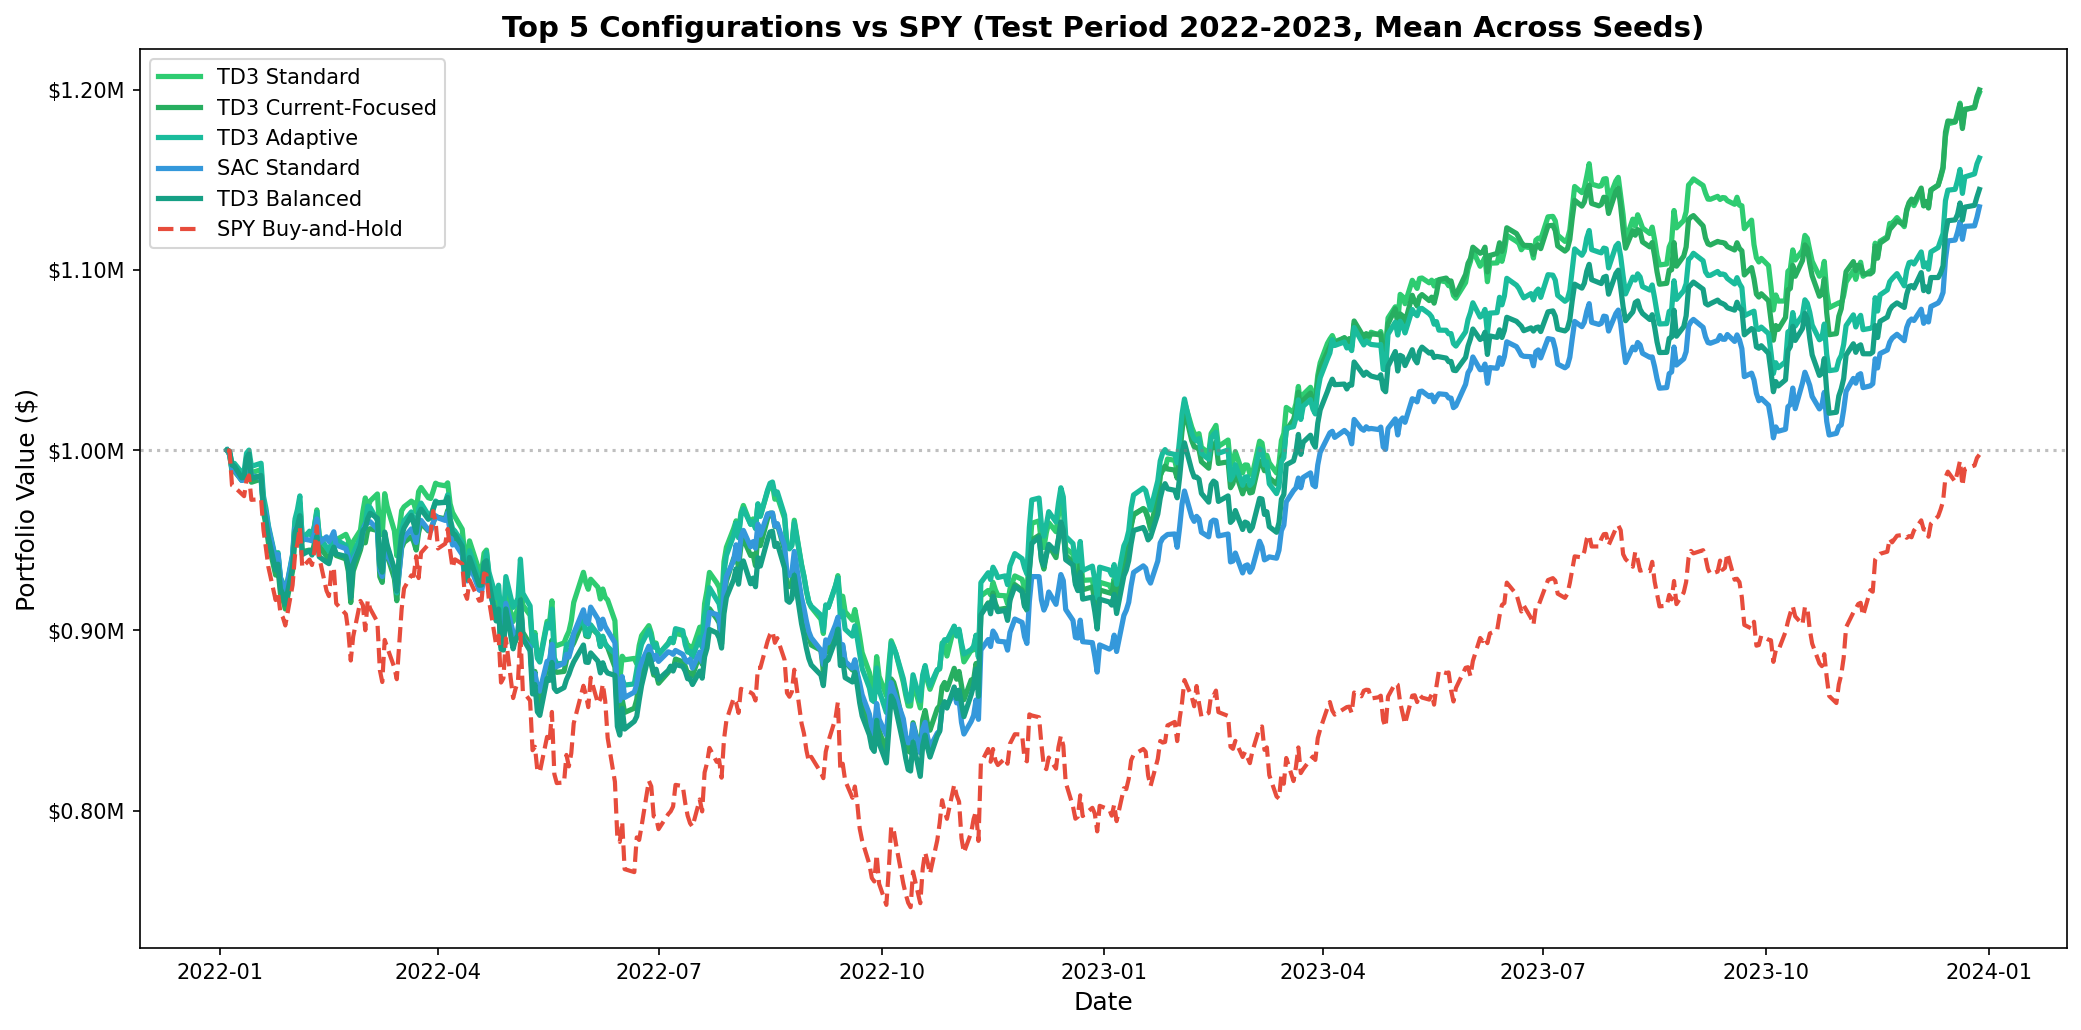
\includegraphics[width=0.78\textwidth]{figures/equity_curves_top5.png}
    \caption{Equity curves for the top 5 algorithm--strategy configurations versus SPY on the 2022--2023 test period (mean across 5 seeds). All configurations outperform SPY, navigating the 2022 drawdown and capitalizing on the 2023 recovery.}
    \label{fig:equity-curve}
\end{figure}

\subsection{SAC Incompatibility with Regime-Aware Replay}

SAC with standard replay achieves $+0.458$, the fourth best configuration, but balanced replay degrades this to $-0.014$. This is a complete loss of profitability. SAC balanced is Bonferroni-significant ($p = 0.002$, $d = -2.95$), while current-focused and inverse-frequency show raw-significant declines ($p < 0.02$, $|d| > 2.0$) that do not survive correction at $\alpha = 0.003$. All four non-standard strategies exhibit large negative effect sizes ($|d| > 1.0$), consistent with systematic degradation rather than random variation (Appendix~D). No other algorithm exhibits this pattern.

We attribute this to SAC's entropy-regularization objective, which assumes training samples reflect the true state-action distribution. \citet{wang2019ere} observed SAC's sensitivity to replay distribution modifications and \citet{saglam2023actor} proved that non-uniform sampling causes actor policy gradients to diverge. Our finding extends these to regime-stratified replay, where the structural rebalancing biases SAC's automatic entropy temperature, leading to miscalibrated exploration. SAC should not be combined with any form of stratified replay without distribution correction.

\begin{figure}[H]
    \centering
    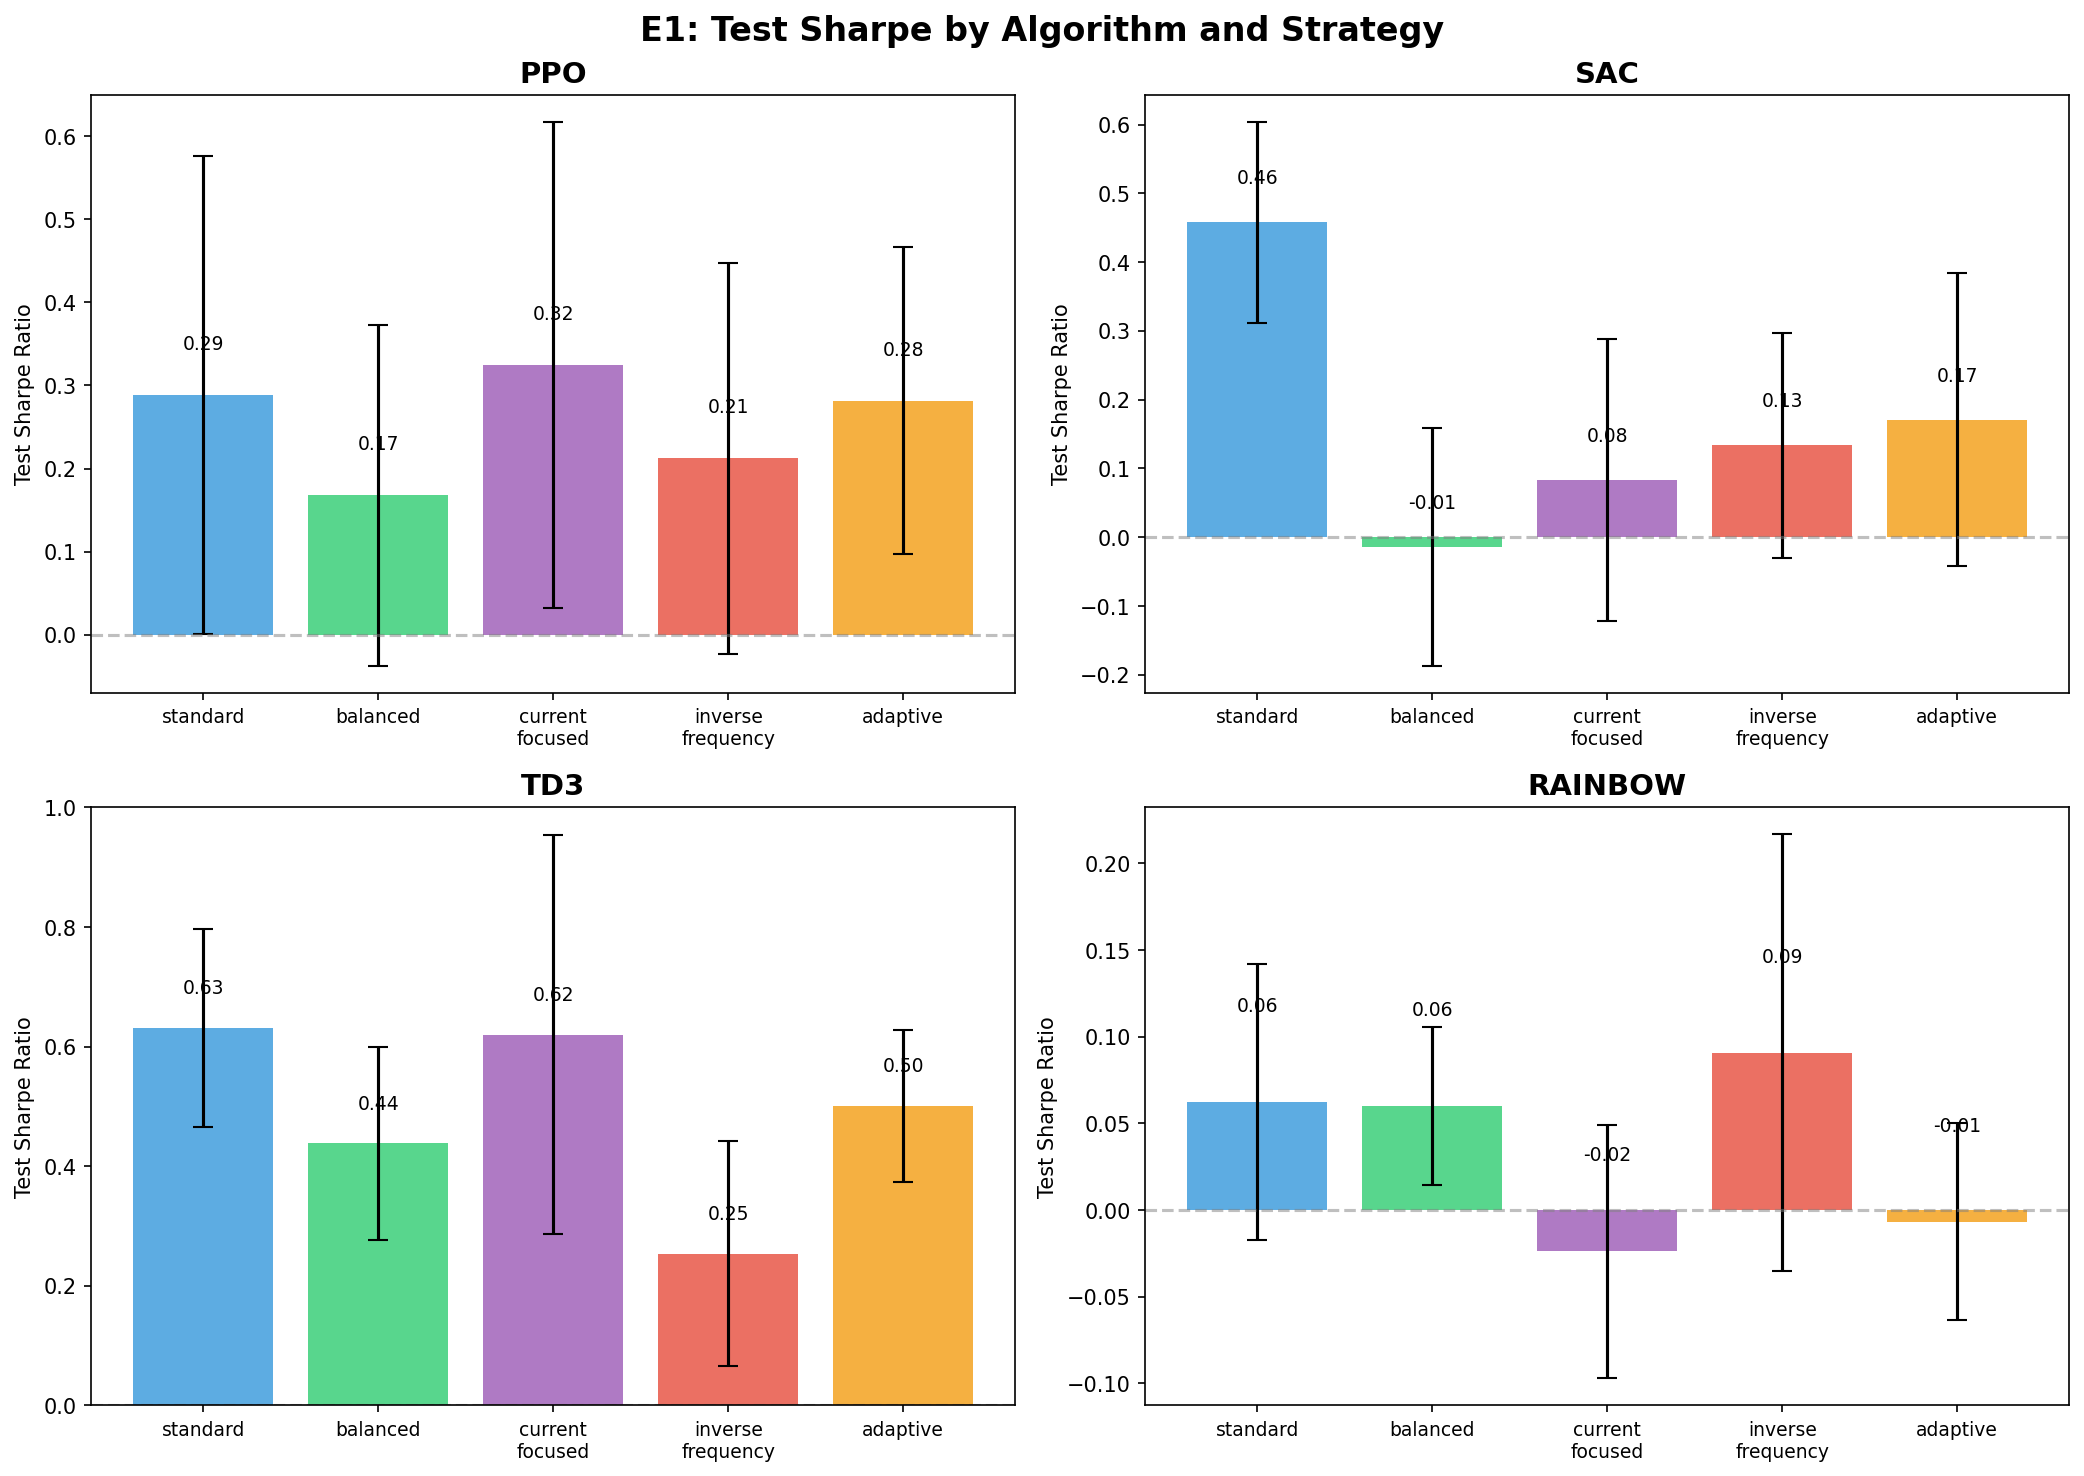
\includegraphics[width=0.82\textwidth]{figures/sharpe_by_strategy_bars.png}
    \caption{Test Sharpe ratios across all algorithm--strategy combinations (E1, 5 seeds per bar). TD3 performs consistently well; SAC collapses with any non-standard replay; Rainbow overfits regardless of strategy.}
    \label{fig:sharpe-bars}
\end{figure}

\subsection{Regime-Level Analysis (E2)}

We decomposed E1 results by market regime (Figure~\ref{fig:regime-heatmap}). Agents profit in bull (mean Sharpe $+1.564$) and bear ($+0.487$) markets but struggle in sideways conditions ($-1.286$). TD3 is the statistically significant bear market champion ($+0.931$ vs PPO $+0.498$, $p < 0.001$, $d = 1.33$; vs SAC $+0.345$, $p < 0.001$, $d = 1.66$), suggesting its deterministic policy gradient suits high-volatility bear dynamics. Counterintuitively, agents \textit{increase} equity allocation in bear markets (46.5\% SPY+QQQ vs 42.4\% in bull), exploiting mean reversion rallies rather than rotating defensively (Appendix~E).

\begin{figure}[H]
    \centering
    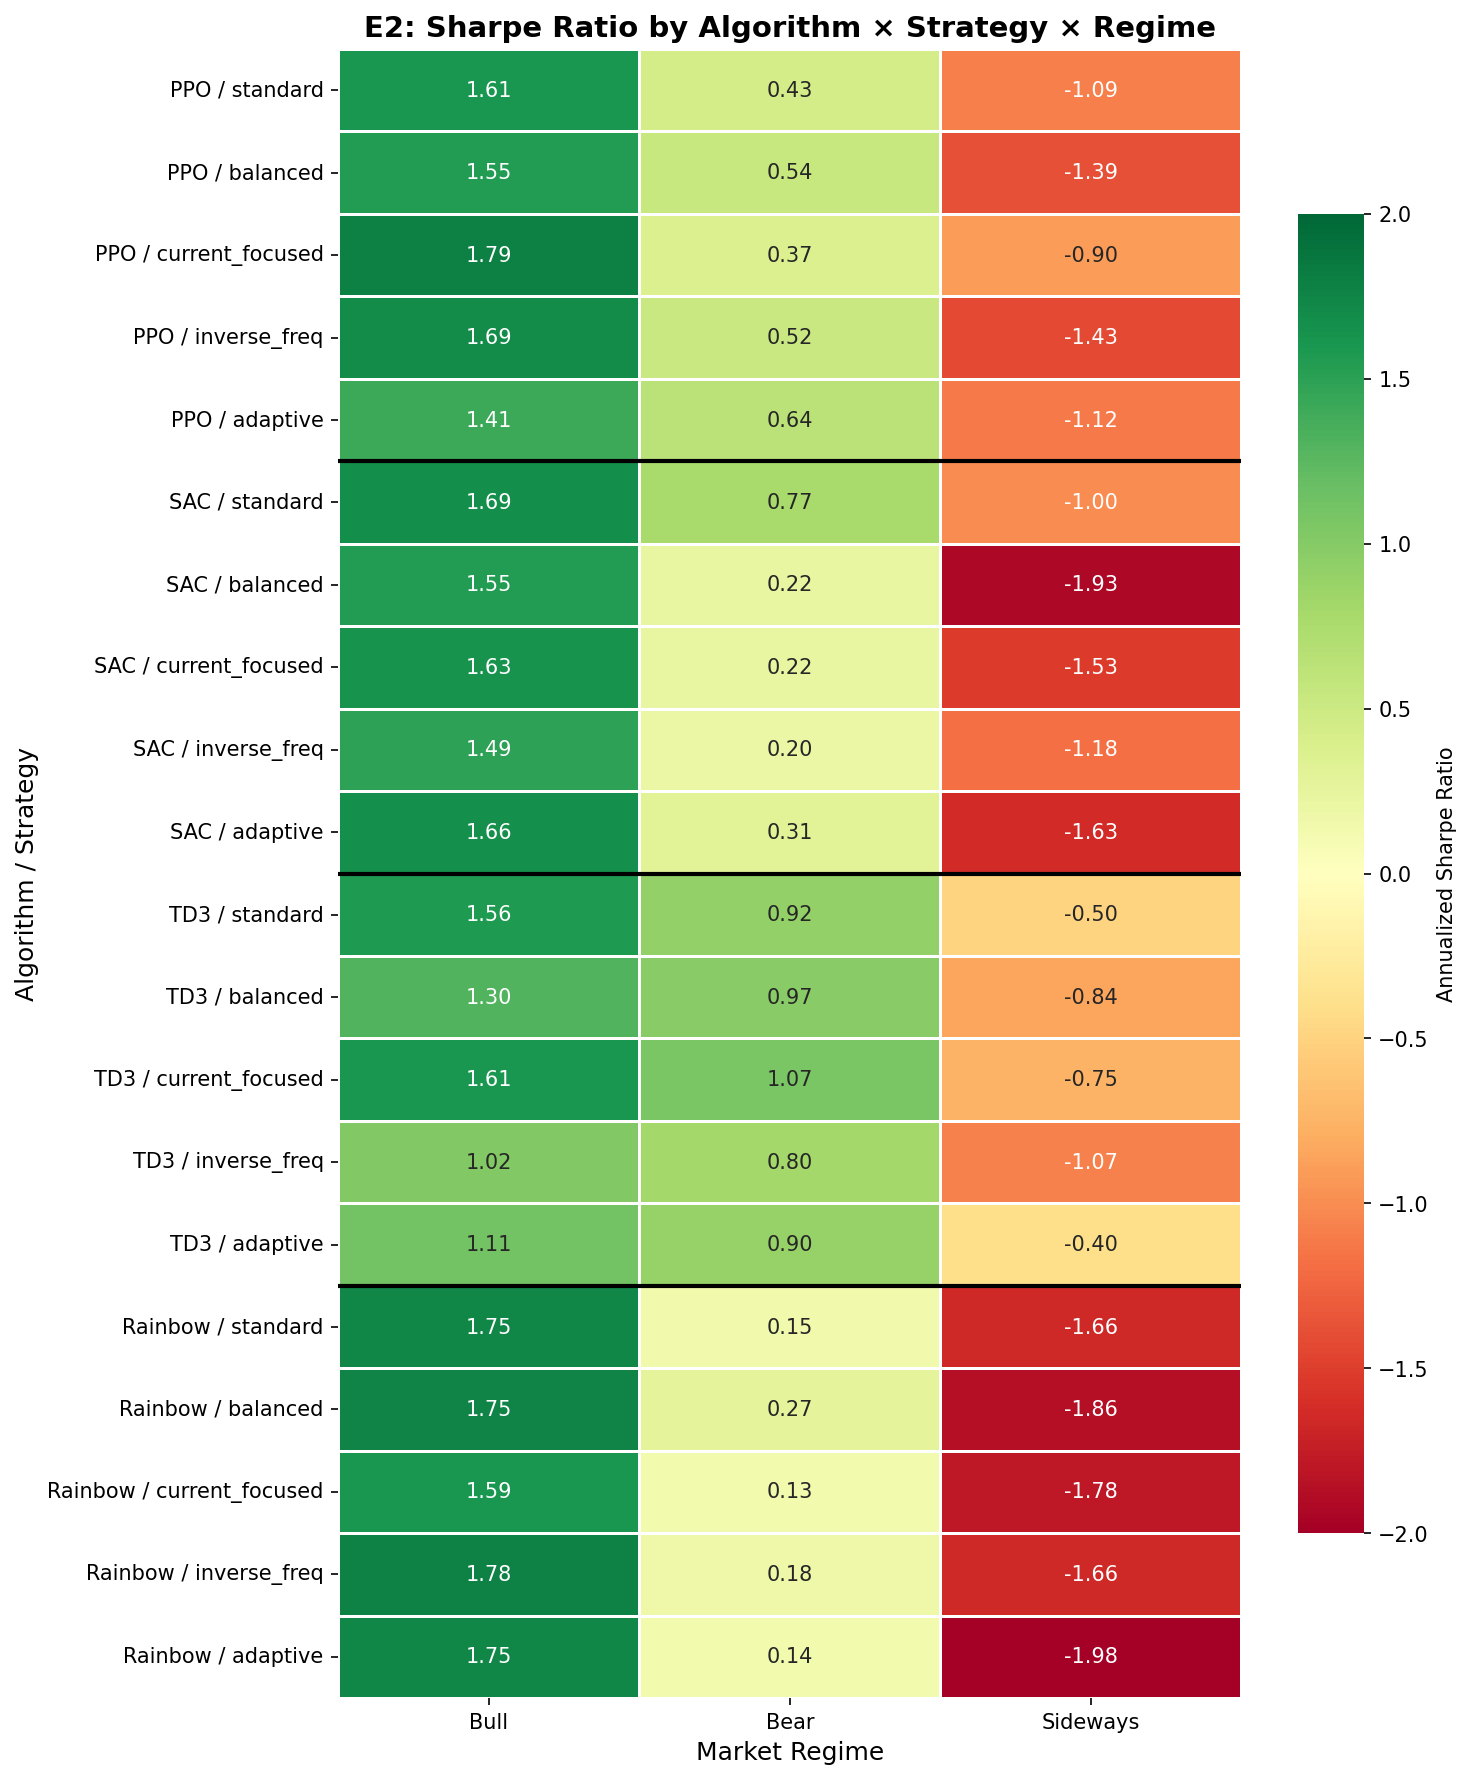
\includegraphics[width=0.82\textwidth]{figures/e2_regime_heatmap.png}
    \caption{Mean test Sharpe by algorithm and market regime (E2). TD3 dominates bear markets; all algorithms struggle in sideways conditions. SAC's poor performance in bear and sideways regimes reflects its sensitivity to non-uniform state distributions.}
    \label{fig:regime-heatmap}
\end{figure}

\subsection{Secondary Experiments (E3--E7)}

Table~\ref{tab:secondary} summarizes the five secondary experiments. The most notable findings are that the approach is robust to imperfect regime detection (E3), that detection method is immaterial even for SAC---the algorithm most sensitive to replay strategy (E5)---and that 400,000 timesteps is the optimal training duration (E7), achieving both the highest test Sharpe and the lowest overfitting gap.

\begin{table}[H]
\centering
\small
\caption{Summary of secondary experiments. Full results in Appendix~C.}
\label{tab:secondary}
\begin{tabular}{@{}clp{5.5cm}@{}}
\toprule
\textbf{Exp} & \textbf{Key Finding} & \textbf{Evidence} \\
\midrule
E3 & Robust to noisy detection & TD3 standard: $+0.652$ at 30\% noise ($p > 0.05$ vs 0\%) \\
E4 & Reduced features preferred & Smaller val--test gap (1.00 vs 1.34 for PPO) with comparable Sharpe \\
E5 & Detection method irrelevant & HMM ($+0.644$) $\approx$ rule-based ($+0.617$) with standard replay \\
E6 & TD3 more sample-efficient & TD3 best: $+0.695$ vs SAC best: $+0.338$ at 1M steps \\
E7 & 400k timesteps optimal & $+0.815$ Sharpe, lowest val--test gap (0.607) \\
\bottomrule
\end{tabular}
\end{table}


\section{Discussion}
\label{sec:discussion}

The central finding of this work is not that any single replay strategy dominates, but that \textit{replay strategy effects are algorithm-dependent}. This is a result with both theoretical and practical implications. TD3 tolerates all five strategies, with standard replay yielding the best performance (Sharpe $+0.632$) followed by current-focused ($+0.620$) and adaptive ($+0.501$). SAC collapses under identical modifications ($d = -2.95$). This asymmetry arises from a fundamental interaction between replay distribution and learning algorithm assumptions. None of the regime-aware strategies significantly outperform standard replay for TD3 ($p > 0.05$), though in bear markets TD3 with current-focused sampling achieves the highest regime Sharpe ($+1.07$ vs $+0.92$ for standard), a practically meaningful difference. Algorithm choice, TD3 over SAC, PPO, or Rainbow, remains the dominant factor \citep{drl_survey2024, hoque2025review}.

The SAC incompatibility is the most consequential result. Prior work has established that SAC is sensitive to replay distribution modifications: \citet{wang2019ere} found that standard PER provides only marginal gains for SAC, \citet{saglam2023actor} proved theoretically that high-TD-error transitions produce policy gradients that diverge from the true gradient in actor-critic methods and \citet{banerjee2024improved} required mixing on-policy data with prioritised replay to stabilise SAC training. Our finding extends this to regime-stratified replay, which imposes a systematic distribution shift. Formally, SAC's temperature update $\alpha^* = \arg\min_\alpha \mathbb{E}_{s \sim \mathcal{D}}[-\alpha \log \pi(a|s) - \alpha \bar{\mathcal{H}}]$ assumes $\mathcal{D}$ approximates the on-policy state visitation $d^\pi(s)$. Under regime-balanced sampling ($P(z) = 1/3$), $\mathcal{D}$ overweights states from rare regimes, inflating entropy estimates and deflating $\alpha$ below its optimal value, causing under-exploration in frequently visited states. The evidence is unambiguous (0\% win rate, $p = 0.002$, $d = -2.95$; Appendix~D). Distribution correction methods \citep{kumar2020discor, sinha2022lfiw} could restore compatibility but would partially counteract regime reweighting.

This finding extends beyond financial DRL: any domain modifying experience replay (curriculum learning, sim-to-real transfer, multi-task RL) must consider whether the learning algorithm's assumptions are violated by the resulting distribution shift.

The current-focused strategy's emphasis on the active regime, and the adaptive strategy's TD-error-guided sampling, conceptually related to DisCor's focus on regions with least-accurate value estimates \citep{kumar2020discor}, help explain TD3's bear market advantage. Agents \emph{increase} equity allocation in bear markets, exploiting mean-reversion rallies rather than adopting a defensive posture. However, this does raise concerns about robustness during prolonged drawdowns. The secondary experiments provide complementary insights: regime detection accuracy and method are immaterial (E3, E5), 400k timesteps optimally balances fit and generalisation (E7) and reduced features perform comparably with less overfitting (E4), consistent with findings from large-scale evaluations \citep{ayari2025feature}.

Returning to our hypotheses (Appendix~B): H1 (regime-aware replay improves returns) is not supported, standard replay remains strongest. H2 (balanced reduces variance) and H3 (inverse-frequency improves bear performance) are unsupported as TD3's bear market dominance is algorithmic. H4 (current-focused aids adaptation) is partially supported, achieving the highest bear regime Sharpe for TD3. H5 (benefits generalise across algorithms) is decisively rejected by the SAC finding. Only H6 (robustness to noisy detection) is fully supported. These mixed results underscore that the investigation’s value lies in revealing how replay and learning interact in an algorithm-dependent manner.

Practitioners should: (i) prefer TD3 over SAC for regime-aware systems, (ii) use 400k rather than 500k timesteps to avoid overfitting and (iii) not invest in sophisticated regime detection; simple rule-based methods suffice.

\textbf{Limitations.} The most consequential is the \textit{single test window}: all out-of-sample results reflect 2022--2023 specifically. Walk-forward validation would strengthen generalisability claims but was infeasible within our data range. \textit{Limited statistical power} ($n = 5$ seeds) means moderate effect sizes may fail to reach significance. Notably, TD3 adaptive vs standard would likely reach significance at $n = 15$, suggesting our non-significant result reflects limited power rather than a true null effect. All configurations exhibit validation--test gaps of 0.6--1.7 Sharpe units, driven by regime mismatch between bull validation (2020--2021) and bearish test (2022--2023); TD3 shows the smallest gaps (0.905--1.354), while Rainbow overfits most severely ($>$1.3). The \textit{correlated equity assets} (SPY--QQQ $\rho > 0.9$) limit diversification and $r_f = 0$ inflates absolute Sharpe ratios, though neither affects the relative ordering of algorithms and strategies. We omit importance sampling corrections, though literature suggests this is minor for regime-level reweighting \citep{fedus2020replay, daley2021stratified}. Future work should employ walk-forward validation, investigate within-regime distribution correction for SAC \citep{li2024roer} and combine replay-based with observation-based regime awareness \citep{nixon2025regime}.

\section{Conclusion}
\label{sec:conclusion}

We investigated whether regime-aware experience replay improves DRL for portfolio optimisation, evaluating five replay strategies across four algorithms in 228 runs with rigorous statistical testing. TD3 with standard replay achieves the best overall performance (Sharpe $+0.632$, Sortino $+0.998$, return $+19.7\%$), though all TD3 configurations outperform baselines. Algorithm choice dominates strategy choice. SAC degrades under all non-uniform replay strategies (Bonferroni-significant, d = -2.95 for balanced), consistent with known sensitivity to replay distribution changes but previously undemonstrated for regime-stratified sampling. The approach is robust to imperfect detection and optimal at 400k timesteps.

These results highlight a general principle: replay buffer modifications must respect learning algorithm assumptions. Entropy-regularised methods are sensitive to distribution shifts that deterministic policy methods tolerate. Regime-aware replay is a lightweight, architecture-agnostic technique suitable for any off-policy algorithm, and combining it with observation-based regime awareness \citep{nixon2025regime} is a promising future direction. Full experimental results and implementation details are in Appendices~A--H.

\setlength{\bibsep}{0.25pt}
{\footnotesize
\bibliographystyle{plainnat}
\bibliography{references}
}

\end{document}
